\documentclass[12pt]{article}
\usepackage{sigsam, amsmath, amssymb} 
% Get sigsam.sty from http://www.sigsam.org/cca/sigsam.sty
\usepackage{url}
%\usepackage{natbib}
\newtheorem{theorem}{Theorem}
\newtheorem{example}{Example}
\newtheorem{definition}{Definition}

\usepackage[moderate]{savetrees}
\usepackage{hyperref}
\usepackage{graphicx}

% leave as is
\issue{vol. 49.1 (March 2015), pp 1--10. }
\articlehead{ACM CCA, vol. 49.1 (March 2015)}
\titlehead{The \textsc{SDEval} Benchmarking Toolkit}
\authorhead{Albert Heinle and Viktor Levandovskyy}
\setcounter{page}{1}

%\reversemarginpar
%\makeatletter \@twosidefalse \makeatother
%\renewcommand*{\marginfont}{\color{red}\bf}
%\newcommand{\TODO}[1]{\marginnote[#1]{}}

%\bibliographystyle{alpha}

\begin{document}

\title{The \textsc{SDEval} Benchmarking Toolkit}

\author{Albert Heinle\\
Cheriton School of Computer Science\\ University of
Waterloo\\ Waterloo, Canada\\\url{aheinle@uwaterloo.ca} \and Viktor Levandovskyy\\
Lehrstuhl D f\"ur Mathematik\\ RWTH
 Aachen University\\ Aachen, Germany\\
\url{levandov@math.rwth-aachen.de}}

% \institute{Cheriton School of Computer Science, University of
%   Waterloo, Waterloo, Canada \and Lehrstuhl D f\"ur Mathematik, RWTH
%   Aachen University, Aachen, Germany}

\maketitle

\begin{abstract}
  In this paper we will present \textsc{SDeval}, a software project that
  contains tools for creating and running benchmarks with a focus on problems
  in computer algebra. It is built on top of the \textsc{Symbolic Data}
  project, able to translate problems in the database into executable code for
  various computer algebra systems. The included tools are designed to be very
  flexible to use and to extend, such that they can be easily deployed even in
  contexts of other communities. We also address particularities of
  benchmarking in the field of computer algebra.

Furthermore, with \textsc{SDEval}, we provide a feasible and automatable way of
reproducing benchmarks published in current research works, which appears to be
a difficult task in general due to the customizability of the available
programs.

\end{abstract}

%%%%%%%%%%%%%%%%%%%%%%%%%%%%%%%%%%%%%%%%%%%%%%%%%%

\section{Introduction}

Benchmarking of software -- i.e. measuring the quality of results and the time
resp. memory consumption for a given, standardized set of examples as input --
is a common way of evaluating implementations of algorithms in many areas of
industry and academia. For example, common benchmarks for satisfiability modulo
theorems (SMT) solvers are collected in the standard library \textsc{SMT-LIB}
\cite{barrett2010smt}, and the advantages of various solvers like \textsc{Z3}
\cite{de2008z3} or \textsc{CVC4} \cite{barrett2011cvc4} are revealed with the
help of those benchmarks.

Considering the field of computer algebra, there could be various benchmarks
for the different computation problems. Sometimes, one can find common problem
instances throughout papers dealing with the same topics, but often there is no
standard collection and authors use examples best to their knowledge. For the
calculation of Gr\"obner bases for example, there is a collection of ideals
that often appear when a new or modified approach accompanied by an
implementation is presented (e.g. in \cite{sneumann2012Parallel}, the author
uses the classical examples \textsc{Katsura}-$n$, $n \in \{11,12\}$, from
\cite{katsura1987distribution} and \textsc{Cyclic}-$m$, $m \in \{8,9\}$, from
\cite{bjorck2008all} to evaluate his new implementation). Regarding the
computation on that set, the new implementation is then compared to existing
and available ones. Note, that even in computations of Gr\"obner bases of
polynomial ideals there are parameters, defining the concrete instance of the
computation task, such as the ground field and the ordering on
monomials. Different computer algebra systems vary in the implemented
functionality, see e.g. \cite{GBImpl} for the comparison.

An outstanding systematic and transparent practice has been shown in 2001 by
the computer algebra lab, lead by V.~P.~Gerdt, of the ``Joint Institute For
Nuclear Research'', on their website about the progress in research of
computing Janet and Gr\"obner bases of complicated polynomial systems
(\url{http://invo.jinr.ru/}).

Nevertheless, in many areas, there is rarely a standard test set, and often the
stated timings and computed results are hard to reconstruct due to different
parameters in algorithms that can be set.

Another difficulty is the fair evaluation on how much time is consumed; we will
discuss this topic detailed in section \ref{sctn:SDEval}.

A database containing a collection of various instances of problems coming
especially from the computer algebra community is given by the \textsc{Symbolic
  Data} project \cite{grabe2006symbolicdata}. It started more than 10 years
ago, and its team of developers is steadily extending the collection of problem
instances together with precise references to their origins. Furthermore, the
ways of accessing the information in the database and interlinking it with
other databases are being kept up to date. For the latter e.g., the techniques
of the so called ``semantic web'' movement have been applied (for more details
consider \cite{grabe2013symbolicdata}). The entries are given in the
\texttt{XML} data format, which makes it easy to parse them since almost every
programming language nowadays provides \texttt{XML} support. All these
arguments lead to the decision to use \textsc{Symbolic Data} as the underlying
database for our project.

We are going to further discuss particularities concerning benchmarking
especially for the computer algebra community and present \textsc{SDEval}, a
benchmarking toolbox written in \textsc{Python} covering the following two main
tasks:
\begin{itemize}
\item[(i)] Creating benchmark sets with the help of the problem instances
  provided by the \textsc{Symbolic Data} database entries.
\item[(ii)] Running benchmarks, with a flexible (i.e. cross-community
  adaptable) interface that makes reproduction as simple as possible.
\end{itemize}

For item (i), we implemented for certain computational problems
(e.g. calculation of a Gr\"obner basis) translators of respective problem
instances from \textsc{Symbolic Data} into executable code for a set of
computer algebra systems.

%% It can be done using a graphical user interface, or alternatively via a
%% program run in the terminal. This task addresses e.g. developers, who want
%% to compare the running time of their implementations with those of available
%% software without the necessity of becoming familiar with all of the
%% available systems. Additionally, it addresses mathematicians who discovered
%% a certain instance for a computational problem and want to examine what
%% computer algebra systems are able to solve it and what solutions are
%% provided, as they might differ -- depending on the uniqueness of the result
%% -- for the different systems.

Item (ii) has a broader range of possible uses. First of all, it provides a way
to run arbitrary programs on different inputs. Optionally, it monitors the
computations and terminates programs automatically if they exceed a user-given
time or memory limit.

%%  Recently, we added the possibility for a user to run a certain number of
%% these programs in parallel.  During the computations, intermediate
%% information on which tasks are currently run and which have already finished
%% is provided, and one can stop calculations manually without having to start
%% the whole process all over again. The information is presented through a
%% generated \textsc{HTML} document and -- for potential automation purposes --
%% through an \textsc{XML} file. We chose for this part a structure that is
%% strongly connected to a folder, which can be shared with others and after a
%% negligible amount of adjustment to another machine, the results can be
%% reproduced.

The results are generated and presented in a transparant and reproducible
way. We envision for the future that \texttt{tar}-balls of the folders
generated by SDEval would be published with computation-focused papers, so that
it becomes easier to verify results of the authors.

There is an intersection between this paper and the preprint
\cite{heinle2013symbolicdata}. In the latter, the main focus was on the
interconnection between \textsc{SDEval} and the \textsc{Symbolic Data} project,
whereas this paper solely focuses on the functionalities and motivations of
\textsc{SDEval}.

This work is structured as follows. Section \ref{sctn:SDEval} will deal with
the design principles and functionalities of \textsc{SDEval}. We will elaborate
on item (i) and (ii) from above and show how one can use and extend/adjust it
to individual computation problems if needed. We will address related work in
Section \ref{sctn:relatedWork} and finish by outlining future tasks in Section
\ref{sctn:Conclusion}.

The current version of the presented toolkit \textsc{SDEval} can be found at
\url{github.com/ioah86/symbolicdata}.  The latest information on
\textsc{Symbolic Data} are available at \url{http://symbolicdata.org}.

Note, that on our own we have used \textsc{SDEval} in our studies with respect
to several ongoing projects, see e.g. \cite{CCHLMSU11},
\cite{heinle2013factorization} and \cite{giesbrecht2014factoring}.

\section{SDEval}
\label{sctn:SDEval}

\subsection{Particularities about Benchmarking in Computer Algebra}

\subsubsection{Challenges.}

Writing benchmarks in the field of computer algebra differs from other
benchmarking tasks. A collection of appearing challenges is the following.
\begin{itemize}
\item Sometimes, the results of computations are not unique; that is, several
  non identically equal outputs can be equivalently correct. It is not always
  possible to find a canonical form for an output. Even if this is the case,
  the transformation of output into the canonical form can be quite
  costly. Moreover, the latter transformation is not necessarily provided by
  every single computer algebra system.
\item Related to the previous item: If an answer is not unique, then the
  evaluation of the correctness of the output is often far from trivial. In
  some cases the correctness-evaluation of certain results is even subject of
  on-going research.
  %%VL to the above: example is truncated inhomogeneous GB
\item The field of computer algebra deals with a large variety of topics, even
  though it can be divided into classes of areas where certain common
  computational problems do appear. Thus, there need to be collections of
  benchmarks, optimally one as a standard for each class. The benchmark
  creation process should be flexible to be applicable in a wide range of
  areas.
\item Considering input formats, many computer algebra systems are going their
  own ways, i.e. for many computation problems, telling the respective system
  what to calculate differ a lot. The source of this problem is that the way of
  representing certain given mathematical objects may also not be unified
  across the community.
\end{itemize}
We tried to address these challenges as much as possible when designing our
toolkit.

In particular, the first item is something that differs the creation of
benchmarks for computer algebra problems from most other fields of studies.

The second item leads to one of the design decisions we made for
\textsc{SDEval}, namely that we provide an interface for decision routines,
%and partially include some serving as an example how they could be added.  and
partially include some of them as examples how such routines could be added.
Then, a particular community can deal with this question based on their
problems, and provide \textsc{SDEval} with the information on what routine to
call to obtain an answer.

\subsubsection{Correct and Feasible Time Measurement.} 

Another seemingly trivial, yet controversial question is the correct time
measure of computations, as mentioned in the introduction. It is very common in
computer algebra systems to provide a time measuring functionality, and many of
the timings provided in papers were calculated using those commands, since it
is easily available.

Nevertheless, this methodology is questionable. Often one cannot verify their
validity due to e.g. their source not being open. Furthermore, sometimes
run-time-benefiting calculations are already done during the initialization
phase; therefore one has to specify clearly where to start the provided time
measurement. If one makes use of the implemented techniques, every program has
to be analyzed in detail to find the correct spot to start the time counting in
order to make the comparison fair. Hence, the use of system-provided time
measuring is not practical for fair comparisons.

%% At this point one can see that using the commands provided by the different
%% computer algebra systems are not practical to use for fair comparisons in a
%% feasible way.

A widely spread method in software development is to run programs with the
\texttt{time} command provided with \textsc{Unix} based operating systems (a
similar program for \textsc{Microsoft Windows} is \texttt{timeit}, contained in
\textsc{Microsoft}s \textsc{Server Resource Toolkit}). Even though the time for
parsing input -- which is in general not the complex part about the
computations done in computer algebra -- would then also being taken into
account, we decided that this method is the best choice for \textsc{SDEval}.

It has also another benefit: We are interested in extracting the timing results
from the output files in an automated way, and there is a standard for
providing timings given by the \textsc{IEEE} standard \texttt{IEEE Std
  1003.2-1992 (``POSIX.2'')}); the \texttt{time} command can be instrumented
using a parameter to provide its output according to this standard. Arranging
this format for the output with the help of the included time measurement
mechanisms in computer algebra systems can be regarded as an infeasible
requirement for a user.

%% would lead to the problem that every execution script has also to contain a
%% part for formatting the timing output correctly. In general, researchers
%% should not have to bother about those technical details, and therefore we
%% would see this as an infeasible requirement.

\subsection{The Creation of a Benchmark Suite}
\subsubsection{Basic Terminology.}

Let us start with defining some terminology we want to use throughout this
section. This will serve the purpose of a better understanding of the design
principles of \textsc{SDEval}.

%% Recall that the creation of benchmarks is built on top of the
%% \textsc{Symbolic Data} project. We will use the abbreviation ``SD-Table''
%% for the respective data tables in the \textsc{Symbolic Data} project. Let us
%% start with stating a more concrete technical definition of the term
%% SD-Table.

\begin{definition}[SD-Table]
\label{def:SD-Table}
\index{SD-Table} An SD-Table denotes a table with computation problems given in
the \textsc{Symbolic Data} project.
\end{definition}

\begin{example}[SD-Table]
An example for an SD-Table is the table that contains instances of ideals in a
polynomial ring over $\mathbb{Q}$ using integer coefficients. These instances
can be used e.g. for Gr\"obner basis computations. The abbreviation chosen by
the \textsc{Symbolic Data} project for this table is \texttt{IntPS}.
\end{example}

\begin{definition}[Problem Instance]
\label{def:ProblemInstance}
\index{Problem Instance} A problem instance is in our context a representation
of a concrete input -- aligned to the \textsc{Symbolic Data} format -- that can
be used for one or more algorithms. The input values for the chosen algorithm
are contained in this problem instance. A problem instance is always contained
in an SD-Table.
\end{definition}

\begin{example}[Problem Instance]
  A problem instance is for example the entry \texttt{Amrhein} (an integer
  polynomial system taken from \cite{amrhein1996walking}) in the SD-Table
  \texttt{IntPS}. It contains the list of variables' names and a collection of
  polynomials forming the generators of the respective ideal. The concrete
  system is shown in Figure \ref{fgr:selectPI}.
\end{example}

\begin{definition}[Computation Problem]
  \label{def:ComputationProblem}
  \index{Computation Problem} A computation problem is a concrete and
  completely specified member of a family of algorithms.  In the context of
  \textsc{SDEval}, it specifies which computations we want to perform on
  certain problem instances.

  A selection of computation problems is already provided in the SD-Table
  \texttt{COMP}. The selection can be extended by the user.
\end{definition}

\begin{example}[Computation Problem]
 A computation problem is for example the computation of a Gr\"obner basis
 given an ideal over a polynomial ring over $\mathbb{Q}$ using the
 lexicographic ordering (abbr. \texttt{GB\_Z\_lp}).
\end{example}

\begin{definition}[Task]
  \label{def:Task}
  \index{Task} A task consists of a computation problem, a selection of problem
  instances that are suitable as inputs for it and a collection of computer
  algebra systems that implement algorithms for the computation problem.
\end{definition}

\subsubsection{Automated Creation of Benchmarks}

Now that we have defined some basic terminology, we will address how a
benchmark suite can be generated using the problem instances given in the
SD-Tables. This part of \textsc{SDEval} addresses e.g. developers, who want to
compare the running time of their implementations with those of available
software without the necessity of becoming familiar with all of the available
systems.  Additionally, it addresses mathematicians who discovered a certain
instance for a computational problem and want to examine what computer algebra
systems are able to solve it and what solutions are provided, as they might
differ -- depending on the uniqueness of the result -- for the different
systems.

The \textsc{SDEval} project contains two \textsc{Python} programs that can do
this job: \texttt{ctc.py} and \texttt{create\_{\allowbreak}tasks\_gui.py}.  The
first one is a command-line program, the second one provides a graphical user
interface.  Those scripts perform the following three steps
\begin{enumerate}
\item The user chooses from a set of currently supported computation problems.

%% The presented set can be extended with a low amount of effort, which makes
%% the tool useful across communities. How this is done will be subject of a
%% later subsection.
  
\item After that, the script collects possible problem instances across the
  SD-Tables and presents them to the user. One can pick the desired problem
  instances that should be included in the benchmark. An illustration of this
  step is given in Figure \ref{fgr:selectPI}.
\item In the last step, besides setting configuration parameters, the user
  selects from a set of computer algebra systems for which it is known that
  they contain implementations of the algorithms that solve the selected
  computation problem. Furthermore, the user enters the calling commands to
  execute those systems on the machine she/he wants the computation to be run.
\end{enumerate}

\begin{figure}
\caption{The selection of the problem instance from integer polynomial systems}
\label{fgr:selectPI}
\begin{center}
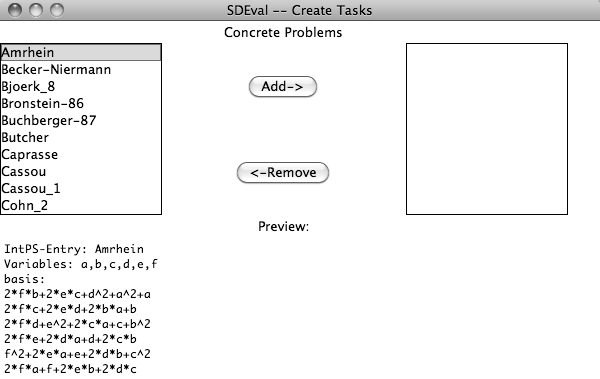
\includegraphics[width=.5\textwidth]{problemSelectionWindow.png}
\end{center}
\end{figure}

After these three steps, the user confirms his or her choices and a folder,
from now on referred to as \textit{taskfolder}, is generated. This folder
containing executable files for the selected computer algebra systems, a
\textsc{Python} script to run all the calculations and some adjustable
configuration files (e.g. if the user wants to change call parameters for a
computer algebra system). The taskfolder can then be sent to the machine where
the computations are intended to be run. The concrete structure is given as in
Figure \ref{fgr:TaskFolder}. As a recent addition, we provided a functionality
that output-analyzing scripts can be included and would automatically be run
after completion of the computation by the computer algebra system. For the
supported computation problems and the supported computer algebra systems, we
already provide scripts to do a light analysis on the output. Light analysis in
this context means that it checks whether there is an output or whether the
calculation has been terminated.

\begin{figure}
\caption{Folder structure of a taskfolder}
\label{fgr:TaskFolder}
{\scriptsize{
\begin{verbatim}
+ TaskFolder 
| - runTasks.py //For Running the task
| - taskInfo.xml //Saving the Task in XML Structure
| - machinesettings.xml//The Machine Settings in XML form 
| + classes //All classes of the SDEval project
| + casSources //Folder containing all executable files
| | + SomeProblemInstance1 
| | | + ComputerAlgebraSystem1
| | | | - executablefile.sdc //Executable code for CAS
| | | | - template_sol.py //Script to analyze the output of the CAS
| | | + ComputerAlgebraSystem2
| | | | - executablefile.sdc
| | | + ...
| | + SomeProblemInstance2
| | | + ...
| | + ...
\end{verbatim}}}
\end{figure}

As outlined before, the creation tool is very flexible and easily
extensible. This is due to the object oriented nature of the code written in
\textsc{Python}. One can specify new computation problems, and declare which
problem instances can be chosen as inputs. The respective code for the computer
algebra systems can be added in a template-fashion and does not require
familiarity with the particular concepts of \textsc{Python}.


\subsection{Running a Benchmark Suite}

\textbf{General Assumption 1:} Whereas the creation of the benchmark suite is
possible on any machine where \textsc{Python} is installed, the running routine
requires a machine running with a \textsc{UNIX}-like operating system
(e.g. \textsc{Linux} or \textsc{Mac OS X}). We require the \texttt{time}
command or some equivalent to be supported, which is in general always the case
on \textsc{UNIX} systems. If one wants to use an equivalent, it needs to be
able to provide an output according to the \textsc{IEEE} standard \texttt{IEEE
  Std 1003.2-1992 (``POSIX.2'')}.

\noindent\textbf{General Assumption 2:} Calculations are run within a
terminal. This decision was made due to the fact that calculations are often
sent to a compute server. The connection to that server is in general provided
through a terminal interface.

The running of a benchmark is closely connected to the taskfolder as presented
in the previous section. As one can see in Figure \ref{fgr:TaskFolder}, it
contains a \textsc{Python} script called \texttt{runTasks.py}. One can either
generate an individual taskfolder using the design principles given in the
documentation (see Figure \ref{fgr:TaskFolder} for the general structure), or
one can use a taskfolder generated by the task creation scripts.

If one executes \texttt{runTasks.py}, all the stored scripts for all the
contained computer algebra systems will be run consequently. Using execution
parameters, one can instruct the script to do the following:
\begin{itemize}
\item Automatically kill a process once a user-provided CPU time limit is
  reached.
\item Automatically kill a process once a user-provided memory consumption
  limit is reached.
\item Run a user-provided number of processes in parallel.
\end{itemize}

\begin{example}
Within a taskfolder, a call of

{\small{\begin{verbatim}$> python runTasks.py -c240 -m100000000 -j4 \end{verbatim}}}%$

\noindent will start the execution process. The computer algebra
systems are terminated if they take more than four minutes to run on a problem
instance (indicated by \texttt{-c240}, where 240 stands for 240s) or if they
use more than approx. 100MB of memory (indicated by \texttt{-m100000000}, where
the unit used is bytes). Futhermore, the user wants to have up to four
processes to be run in parallel (indicated by \texttt{-j4}).
\end{example}

The script will create --- if not yet existent --- a sub-folder within the
taskfolder named \texttt{results}. Within \texttt{results}, there will be a
folder named by the time stamp when \texttt{runTasks.py} was executed, where it
will store the results of the computations, some monitoring information about
the executed scripts (in form of \textsc{HTML} and \textsc{XML} files) and
files containing information about the machine where the calculation is run on
(detailed information on CPU, memory and operating system).

During the execution process, the user can feel free to terminate manually a
running process without having to restart \texttt{runTasks.py}. It will simply
continue with the next waiting program on the next script in the queue. If an
output analyzing script is provided, there will be an error indicated in the
\textsc{HTML} resp. \textsc{XML} table afterwards. Otherwise it will be just
marked as ``completed''.

This design of the benchmark execution part has the following benefit. Future
authors that execute their scripts on certain files could provide their
taskfolder with the paper they submitted. Then everyone can see the results
(i.e. the outputs of the programs), and verify the timings using the calculated
table. Furthermore, they can run the calculation using \texttt{runTasks.py}
after adjusting the configuration to their machine (i.e. replacing the call
commands for the computer algebra systems to those used on one's machine). We
are already adapting this practice, as one can find the timings of the papers
\cite{giesbrecht2014factoring} and \cite{heinle2013factorization} on one of our
personal websites
(\url{https://cs.uwaterloo.ca/~aheinle/software_projects.html}).

%% \subsubsection{Further Uses of the Running Routines.}

There are further uses of the running routines. As we can see, the execution of
the benchmarks is completely detached from the creation part. This means, that
a customized taskfolder can be created, defining programs one wants to run and
provide the inputs and scripts to analyse the outputs inside the
\texttt{casSources} folder.

Even though the routines were designed to fit especially the needs of the
computer algebra community, the principles can be used for almost any kind of
program.

Another use of the taskfolder and the contained \textsc{Python}-program would
be to keep track of the development process of a software project over
time. Executing the \texttt{runTasks.py} script after every version change
would reveal profiling information on the different examples. The profiling can
be automatized since the timing-data after every run is stored in an
\textsc{XML} file.

The following examples will illustrate the flexibility and the ease of
adjustment of the taskfolder.

\begin{example}
  Assume the user already has a taskfolder. Now, he or she encounters a new,
  interesting problem instance and intends to add it to the existing problem
  instances in the taskfolder. There are two ways of doing it:
  \begin{itemize}
  \item If the user is familiar with every computer algebra system that is used
    in this taskfolder, the user creates the respective scripts and adds the
    problem with the scripts as a new subfolder to \texttt{casSources}.

      %% he or she can copy and paste one of the subfolders of
      %% \texttt{casSources}, rename it, and change the input of the files in
      %% the respective subfolders representing the computer algebra systems.

    Then, it remains to add an entry in the \texttt{taskInfo.xml} file. In
    particular, the entry is given by the following lines:
\begin{verbatim}
<probleminstance>
  myNewExample
</probleminstance>
\end{verbatim}
  After that, the example will be considered with the next run.
  \item If the user is not familiar with the computer algebra systems in use,
    then an entry in the database of \textsc{Symbolic Data} has to be made,
    which is a simple \textsc{XML} file. After that, the user can use our tool
    to automatically generate code for the computer algebra systems that have
    functionality for the respective computation problem.
  \end{itemize}
\end{example}

\begin{example}
  As in the previous example, assume that the user is already in possession of
  a taskfolder. Now he or she wants, in addition to the considered computer
  algebra systems, benchmark a personal, maybe self written program on the
  examples. All the user has to do is then generate for every problem instance
  in the folder \texttt{casSources} a subfolder with the respective
  script. After that, the user specifies how the program is called (parameters,
  options, etc.) in the \texttt{MachineSettings.xml} file, registers it in the
  \texttt{taskInfo.xml} and then the program will be considered in the next
  call of \texttt{runTasks.py}.
\end{example}

\begin{example}
By using SDEval ourselves, we also have encountered the following scenario. We
generated a taskfolder with a large set of problem instances. After running the
computer algebra systems on these problem instances, we realized that currently
some cannot be solved in a feasible amount of time. Thus, until there is a new
version of one of the used computer algebra systems, we want to exclude the
example when executing \texttt{runTasks.py}. This can be done by simply
commenting out the respective entries in the \texttt{taskInfo.xml} file.

The same can be done to a computer algebra system which performs poorly in
comparison to others, i.e. the user can comment it out until a new version
appears.
\end{example}

\subsection{Ways of Customizing and Contributing to \textsc{SDEval}}

We have seen in the last section that the part of the execution of the
respective programs on the problem instances is highly customizable. There are
also ways for customization of the part where one creates benchmarks.

%% In this subsection we will show
%% \begin{itemize}
%% \item how a user familiar with a computer algebra system, which is not
%%   considered for a certain computation problem yet, is able to provide a
%%   template to create executable and optionally output-analyzing code without
%%   the need of a deep knowledge of \textsc{Python},
%% \item how a user can add a new computation problem for which inputs can be
%%   derived from existing SD-tables and
%% \item how a user can add new problem instances to the \textsc{Symbolic Data}
%%   database.
%% \end{itemize}

\subsubsection{Adding Templates for Computer Algebra Systems.}

 The templates can be found in the folder \texttt{templates} in the
 \textsc{SDEval} project. One simply has to add a new folder named after the
 new computer algebra system, and within this folder there must be a file with
 the function that generates the code. Optionally, one can also write a script
 that analyzes the output of the respective computer algebra system. The
 function headers themselves can be copied from the other, already available
 templates, and one only has to adjust the respective code lines for the
 computer algebra system one wants to add. For this, there is no deep knowledge
 of \textsc{Python} needed. For more details consider the Q\&A file in the
 documentation.

\begin{example}
  Let us consider a possible template for \textsc{Singular} to create
  executable code to calculate a Gr\"obner basis using the lexicographic
  ordering for a given problem instance coming from the SD-Table
  \texttt{IntPS}:
  \begin{verbatim}
def generateCode(vars, basis):
    """
    [Documentation lines]
    """
    result = """
ring R = 0,(%s),lp;
ideal I = %s;
ideal J = std(I);
print(J);\n\
$
""" % (",".join(vars),",\n".join(basis))
    return result
 \end{verbatim}%$
As one can see, all it takes is to create a formatted string, and the
respective values will be provided by the input parameters of the function
\texttt{generateCode}, which is the standardized in \textsc{SDEval}.
\end{example}

\subsubsection{Adding New Sets of Problem Instances.}

Communities can add new tables with problem instances into the \textsc{SDEval}
project. For associating it with a given computation problem, this table has to
be added to the supported sets of a computation problem within the project.

\subsubsection{Adding New Computation Problems.}

New computation problems can be divided into two kinds: the ones where the
inputs of respective algorithms can be derived from existent tables, and the
ones where in addition new sets of problem instances have to be added. The
latter category requires more work. For the first one, a user can either choose
the way of writing a representative class for the computation problem within
the \textsc{SDEval} project, or contact the project team with an request to add
this computation problem to \textsc{SDEval} due to its importance.


%Notes:
% - Subsection about principles of testing
% - Subsection: ``The Creation Process''
% - (Sub-)Subsection: ``How to Extend the functionality''
% - Subsection: ``The Running Process''
% - Mention that this can also be used as a way to let
%        other people reproduce the computation results
%        of an author of a paper.
% - Fairness of timings


%%%%%%%%%%%%%%%%%%%%%%%%%%%%%%%%%%%%%%%%%%%%%%%%%%

\section{Related Work}
\label{sctn:relatedWork}

\textsc{StarExec} \cite{stump2012introducing}: This is an infrastructure
especially for the logic solver communities. Its main focus is to provide a
platform for managing benchmark libraries and run solver competitions. It is
widely used in conferences based on logic solving to evaluate the benefits of
new approaches. Moreover, it includes translators of problems between the
different communities dealing with logic solving. Calculations are always run
on the same hardware, therefore results can directly be compared to all other
benchmarks that were run before without taking hardware differences into
consideration. The main difference to our project is that it provides less
flexibility for the individual researcher to define customized computation
problems and submit problem instances. Furthermore, as the input data comes
from the logic solver community, the input is standardized and every program
accepts the same types of files. For computer algebra systems, this is
different, as stated earlier.

%%  Consider as an example the definition of a Gr\"obner Basis; there is no
%% standardized input way that all computer algebra systems accept, thus those
%% input files are different.

\textsc{homalg} \cite{barakat2008homalg}: Focusing on constructive homological
algebra, the \textsc{homalg} project provides an abstract structure for abelian
categories and is distributed as a package of the computer algebra system
\textsc{GAP} \cite{GAP4}. For time critical computations, it allows the usage
of other computer algebra systems, i.e. the task is translated to the
respective system and then executed.  This corresponds to the translation part
of the \textsc{SDEval} project for the supported computation problems.

\textsc{Sage} \cite{stein2008sage}: The popular computer algebra system
\textsc{Sage} provides as an optional package an interface to the database of
integer polynomial systems (\texttt{IntPS}) of the \textsc{Symbolic Data}
project. One can directly load those problem instances as objects in
\textsc{Sage} for further calculations and apply the implemented/wrapped
algorithms on them.

%% \subsection{Related Work to \textsc{Symbolic Data}}

%% There are various sets of problem instances for different computation
%% problems collected by different communities during the last couple of
%% decades. Here is a selection of some interesting projects.

%% \textsc{PoCab} \cite{samal2012pocab}: \textsc{PoCab} is a collection
%% of models coming from the field of biology and chemistry. They
%% concentrate on examining the different algebraic entities given in
%% those models in order to apply algebraic methods in the process of
%% their analysis. Their data of interest is coming from two renowned and
%% publicly available databases, namely \textsc{KEGG}
%% \cite{kanehisa2000kegg} and the \textsc{Biomodels Database}
%% \cite{le2006biomodels}.

%% \textsc{Polytope Database}
%% (\url{www.mathematik.tu-darmstadt.de/~paffenholz/data.html}): 
%% At the third annual meeting of the DFG Priority Project SPP 1489, which was
%% held from March 18 to 22 in Konstanz, Germany, the \textsc{Symbolic Data}
%% team established an interesting contact, namely to Dr. Andreas
%% Paffenholz. He Dr. Andreas Paffenholz (TU Darmstadt) has a large amount of
%% resource data as {\sc Polymake} files for different kinds of polytopes. It
%% will be extracted and possibly there will soon be metadata generated and
%% included into \textsc{Symbolic Data}.

%% \textsc{swMATH} (\url{http://swmath.org}): The focus of this project
%% is to serve as an information service for mathematical software. It
%% consists of an extensive database of software projects from the field
%% of mathematics, and contributes a systematic linking of program
%% packages with relevant publications.

%% \textsc{Qaos} (\url{http://qaos.math.tu-berlin.de}): This project at the TU
%% Berlin is the successor of the ``Kant Database of Number Fields''. It
%% provides an interface to various categories of algebraic objects.  Not only
%% it provides a web interface to access the data, it also provides interfaces
%% for a selection of computer algebra systems. This part makes it also related
%% to the task creation process of \textsc{SDEval}.

%% %Notes:
%% % - Mention starExec

%%%%%%%%%%%%%%%%%%%%%%%%%%%%%%%%%%%%%%%%%%%%%%%%%%

\section{Conclusion and Future Work}
\label{sctn:Conclusion}

We have presented a benchmarking tool named \textsc{SDEval}, which is built on
top of the \textsc{Symbolic Data} project. In this paper, we addressed the
particularities of benchmarking in the field of computer algebra, and with
\textsc{SDEval}, we have presented a flexible, extensible and easy-to-use tool
that is designed to accept the challenge.

Moreover, we introduced a practice how the reproduction and the analysis of
computations with their timings would become more feasible in the future.  Our
approach for that is the taskfolder containing the benchmark program and the
respective input files.

A future task will be to extend the benchmark creation tool to contain both
more computer algebra systems and computation problems. As we have outlined in
the paper, these extensions are easy tasks due to the chosen design of
\textsc{SDEval}.  The output interpretation routines are very basic at the
current stage. In fact, they are just checking if feasible output can be
extracted or not. In the future, we plan to implement thorough tests with which
one can determine the correctness of the outputs. For that, one has to consider
every computation problem in a detailed way and we hope for support from the
communities to accomplish that.

Further possibilities and details about how to customize SDEval can be found in
the documentation of \textsc{SDEval}. We would be happy to receive
contributions and suggestions from users.  But of course, even though we tried
to simplify the processes of contributing as much as we could, it would take
time from a person outside the project to obtain a basic understanding of the
whole system.  If one is not willing to contribute for this reason, but would
like to see certain additions to the toolkit, please contact the authors. We
are very thankful for any kind of input that can help to extend the
functionality of \textsc{SDEval}.

About the timing-results of a benchmark, we plan to write a toolset to analyze
these. By now, the timings that we are collecting are saved within
\textsc{XML}-files. One can use this information to draw trends when applying
different versions of computer algebra systems for example. An environment
close to a testing-suite is on the agenda of the \textsc{SDEval} project.

As benchmarking is a very wide-ranged topic, we will continuously consider
further challenges -- maybe caused by not yet considered computation problems
-- that we have not dealt with in the present state.  It remains a practically
relevant and interesting problem.

\section*{Acknowledgements}

We thank the ``Deutsche Forschungsgesellschaft'' (DFG) for partial financial
support for the development of \textsc{SDEval} (``DFG Priority Project SPP
1489'').  in the context of the ``DFG Priority Project SPP 1489: Algorithmic
and Experimental Methods in Algebra, Geometry and Number Theory.''

%% Also, we would like thank the ``Europ\"aische Sozialfonds f\"ur
%% Deutschland'' (ESF) for partially funding the work on \textsc{Symbolic Data}
%% in the context of the project ``eScience – Forschungs\-netz\-werk Sachsen''.
%% Moreover we personally thank Dr.~Toni Tontchev (HTWK Leipzig) for his
%% enthusiastic support.

The authors are especially grateful to Prof.~Dr.~Hans-Gert Gr\"abe
(Universit\"at Leipzig), the major maintainer of {\sc SymbolicData} project,
for his encouragement and the numerous fruitful discussions we had with
him. Moreover, we thank Andreas Nareike (Leipzig) for valuable discussions and
Benjamin Schnitlzer (Aachen) for his collaboration on the {\sc SDEval} project.

The authors thank Prof.~Dr.~Johannes Waldmann (HTWK Leipzig) for his
introduction to the benchmarking practices of the logic solver communities
during the \textsc{Symbolic Data} workshop.

Special thanks go to Prof.~Dr.~Mark Giesbrecht (University of Waterloo) for his
helpful suggestions and valuable comments.

%%%%%%%%%%%%%%%%%%%%%%%%%%%%%%%%%%%%%%%%%%%%%%%%%%

%\bibliographystyle{alpha}
%\bibliography{sdeval}
\begin{thebibliography}{21}
\providecommand{\etalchar}[1]{$^{#1}$}
%\providecommand{\natexlab}[1]{#1}
%\providecommand{\url}[1]{\texttt{#1}}
%\expandafter\ifx\csname urlstyle\endcsname\relax
%  \providecommand{\doi}[1]{doi: #1}\else
 % \providecommand{\doi}{doi: \begingroup \urlstyle{rm}\Url}\fi

\bibitem[BST10]{barrett2010smt} Clark Barrett, Aaron Stump, and Cesare Tinelli.
  \newblock The smt-lib standard: Version 2.0.  \newblock In \emph{Proceedings
    of the 8th International Workshop on Satisfiability Modulo Theories
    (Edinburgh, England)}, volume~13, 2010.
\bibitem[DMB08]{de2008z3} Leonardo De~Moura and Nikolaj Bj{\o}rner.  \newblock
  Z3: An efficient {SMT} solver.  \newblock In \emph{Tools and Algorithms for
    the Construction and Analysis of Systems}, pages 337--340. Springer, 2008.
\bibitem[BCD{\etalchar{+}}11]{barrett2011cvc4} Clark Barrett,
  Christopher~L. Conway, Morgan Deters, Liana Hadarean, Dejan Jovanovi{\'c},
  Tim King, Andrew Reynolds, and Cesare Tinelli.  \newblock Cvc4.  \newblock In
  \emph{Computer Aided Verification}, pages 171--177. Springer, 2011.
\bibitem[Neu12]{sneumann2012Parallel} Severin Neumann.  \newblock Parallel
  reduction of matrices in {G}r{\"o}bner bases computations.  \newblock In
  Vladimir~P. Gerdt, Wolfram Koepf, Ernst~W. Mayr, and Evgenii~V.  Vorozhtsov,
  editors, \emph{Computer Algebra in Scientific Computing}, volume 7442 of
  \emph{Lecture Notes in Computer Science}, pages 260--270. Springer Berlin
  Heidelberg, 2012.  \newblock URL
  \url{http://dx.doi.org/10.1007/978-3-642-32973-9_22}.
\bibitem[KFI{\etalchar{+}}87]{katsura1987distribution} S.~Katsura, W.~Fukuda,
  S.~Inawashiro, N.~M. Fujiki, and R.~Gebauer.  \newblock Distribution of
  effective field in the {I}sing spin glass of the $\pm j$ model at {$T= 0$}.
  \newblock \emph{Cell Biophysics}, 11\penalty0 (1):\penalty0 309--319, 1987.
\bibitem[BH08]{bjorck2008all} Goran Bjorck and Uffe Haagerup.  \newblock All
  cyclic p-roots of index 3, found by symmetry-preserving calculations.
  \newblock \emph{arXiv preprint arXiv:0803.2506}, 2008.
\bibitem[LRP07]{GBImpl} V.~Levandovskyy, C.~Rosenkranz, and T.~Povalyayeva.
  \newblock Online database {\it gr{\"o}bner bases implementations.
    {f}unctionality {c}heck and {c}omparison}, 2007.  \newblock URL
  \url{http://www.risc.uni-linz.ac.at/Groebner-Bases-Implementations/}.
\bibitem[Gr{\"a}09]{grabe2006symbolicdata} Hans-Gert Gr{\"a}be.  \newblock The
  {\sc SymbolicData} project.  \newblock Technical report, Technical report
  (2000-2009), 2009.  \newblock URL \url{http://www. symbolicdata.org}.
\bibitem[GNJ13]{grabe2013symbolicdata} Hans-Gert Gr{\"a}be, Andreas Nareike,
  and Simon Johanning.  \newblock The {\sc SymbolicData} project--towards a
  computer algebra social network.  \newblock 2013.
\bibitem[HLN13]{heinle2013symbolicdata} Albert Heinle, Viktor Levandovskyy, and
  Andreas Nareike.  \newblock {\sc SymbolicData: SDEval} - benchmarking for
  everyone.  \newblock \emph{arXiv preprint arXiv:1310.5551}, 2013.
\bibitem[CCH{\etalchar{+}}11]{CCHLMSU11} Svetlana Cojocaru, Alexandru
  Colesnicov, Albert Heinle, Viktor Levandovskyy, Ludmila Malahov, Grischa
  Studzinski, and Victor Ufnarovski.  \newblock Creation of a knowledge
  framework for non-commutative computer algebra.  \newblock In \emph{Proc. 7th
    International Conference on Microelectronics and Computer Science,
    Chi\c{s}in\u{a}u, Republic of Moldova}, pages 166--169, 2011.
\bibitem[HL13]{heinle2013factorization} Albert Heinle and Viktor Levandovskyy.
  \newblock Factorization of $\mathbb{Z}$-homogeneous polynomials in the first
  $(q)$-{W}eyl algebra.  \newblock \emph{arXiv preprint arXiv:1302.5674}, 2013.
\bibitem[GHL14]{giesbrecht2014factoring} Mark Giesbrecht, Albert Heinle, and
  Viktor Levandovskyy.  \newblock Factoring linear differential operators in
  $n$ variables.  \newblock In \emph{Proceedings of the 39th International
    Symposium on Symbolic and Algebraic Computation}, pages 194--201. ACM,
  2014.
\bibitem[AGK96]{amrhein1996walking} Beatrice Amrhein, Oliver Gloor, and
  Wolfgang K{\"u}chlin.  \newblock Walking faster.  \newblock In \emph{Design
    and Implementation of Symbolic Computation Systems}, pages
  150--161. Springer, 1996.
\bibitem[SST12]{stump2012introducing} Aaron Stump, Geoff Sutcliffe, and Cesare
  Tinelli.  \newblock Introducing {S}tar{E}xec: a cross-community
  infrastructure for logic solving.  \newblock \emph{Comparative Empirical
    Evaluation of Reasoning Systems}, page~2, 2012.
\bibitem[BR08]{barakat2008homalg} Mohamed Barakat and Daniel Robertz.
  \newblock {\sc homalg} --- a meta-package for homological algebra.  \newblock
  \emph{Journal of Algebra and its Applications}, 7\penalty0 (03):\penalty0
  299--317, 2008.
\bibitem[GAP13]{GAP4} GAP.  \newblock \emph{{GAP -- Groups, Algorithms, and
    Programming, Version 4.6.3}}.  \newblock The GAP~Group, 2013.  \newblock
  URL \url{http://www.gap-system.org}.
\bibitem[S{\etalchar{+}}08]{stein2008sage} William Stein et~al.  \newblock {\sc
  Sage}: Open source mathematical software, 2008.  \newblock URL
  \url{http://www.sagemath.org}.
\bibitem[SEW12]{samal2012pocab} Satya~Swarup Samal, Hassan Errami, and Andreas
  Weber.  \newblock {PoCaB}: a software infrastructure to explore algebraic
  methods for bio-chemical reaction networks.  \newblock In \emph{Computer
    Algebra in Scientific Computing}, pages 294--307.  Springer, 2012.
\bibitem[KG00]{kanehisa2000kegg} Minoru Kanehisa and Susumu Goto.  \newblock
  {KEGG}: {K}yoto encyclopedia of genes and genomes.  \newblock \emph{Nucleic
    acids research}, 28\penalty0 (1):\penalty0 27--30, 2000.
\bibitem[LNBB{\etalchar{+}}06]{le2006biomodels} Nicolas Le~Novere, Benjamin
  Bornstein, Alexander Broicher, Melanie Courtot, Marco Donizelli, Harish
  Dharuri, Lu~Li, Herbert Sauro, Maria Schilstra, Bruce Shapiro, et~al.
  \newblock {BioModels} {D}atabase: a free, centralized database of curated,
  published, quantitative kinetic models of biochemical and cellular systems.
  \newblock \emph{Nucleic acids research}, 34\penalty0 (suppl 1):\penalty0
  D689--D691, 2006.
\end{thebibliography}

\end{document}
